

\documentclass[10pt,a4]{article}
\usepackage[top=0.85in,left=.75in,footskip=0.75in]{geometry}

% amsmath and amssymb packages, useful for mathematical formulas and symbols
\usepackage{amsmath,amssymb}

% Use adjustwidth environment to exceed column width (see example table in text)
\usepackage{changepage}

% Use Unicode characters when possible
\usepackage[utf8x]{inputenc}

% textcomp package and marvosym package for additional characters
\usepackage{textcomp,marvosym}

% cite package, to clean up citations in the main text. Do not remove.
\usepackage{cite}

% Use nameref to cite supporting information files (see Supporting Information section for more info)
\usepackage{nameref,hyperref}

% line numbers
\usepackage[right]{lineno}

% ligatures disabled
\usepackage{microtype}
\DisableLigatures[f]{encoding = *, family = * }

% color can be used to apply background shading to table cells only
\usepackage[table]{xcolor}

% array package and thick rules for tables
\usepackage{array}

% multirow for multiple row tables. 
\usepackage{multirow}

\usepackage{subfig}



% Bold the 'Figure #' in the caption and separate it from the title/caption with a period
% Captions will be left justified
\usepackage[aboveskip=1pt,labelfont=bf,labelsep=period,justification=raggedright,singlelinecheck=off]{caption}
\renewcommand{\figurename}{Fig}

% Use the PLoS provided BiBTeX style
\bibliographystyle{plos2015}

% Remove brackets from numbering in List of References
\makeatletter
\renewcommand{\@biblabel}[1]{\quad#1.}
\makeatother



% Header and Footer with logo
\usepackage{lastpage,fancyhdr,graphicx}
\DeclareGraphicsExtensions{.pdf,.png}   
\usepackage{epstopdf}


\renewcommand\thefigure{S\arabic{figure}} 
\renewcommand\thetable{S\arabic{table}} 
%% END MACROS SECTION


\begin{document}
\vspace*{0.2in}

% Title must be 250 characters or less.
\begin{flushleft}
{\Large
\textbf\newline{Supplementary Material: Joint modelling of aggregated incidence data and point prevalence surveys for malaria mapping} % Please use "sentence case" for title and headings (capitalize only the first word in a title (or heading), the first word in a subtitle (or subheading), and any proper nouns).
}
\newline
% Insert author names, affiliations and corresponding author email (do not include titles, positions, or degrees).
\\
Tim C.D. Lucas*\textsuperscript{1}, 
Anita K. Nandi\textsuperscript{1},
Elisabeth G. Chestnutt\textsuperscript{1},
Katherine A. Twohig\textsuperscript{1},
Suzanne H. Keddie\textsuperscript{1},
Emma L. Collins\textsuperscript{1},
Rosalind E. Howes\textsuperscript{1},
Michele Nguyen\textsuperscript{1},
Susan F. Rumisha\textsuperscript{1},
Andre Python\textsuperscript{1},
Rohan Arambepola\textsuperscript{1},
Amelia Bertozzi-Villa\textsuperscript{1,2},
Penelope Hancock\textsuperscript{1},
Punam Amratia\textsuperscript{1},
Katherine E. Battle\textsuperscript{1},
Ewan Cameron\textsuperscript{1},
Peter W. Gething\textsuperscript{1, 3, 4}
Daniel J. Weiss\textsuperscript{1}
\\
\bigskip
1. BDI, Oxford\\
2. Institute for Disease Modeling, Bellevue, WA, USA\\
3. Telethon Kids Institute, Perth Children’s Hospital, Perth, Australia\\
4. Curtin University, Perth, Australia
\\
\bigskip

\end{flushleft}



% Insert additional author notes using the symbols described below. Insert symbol callouts after author names as necessary.
% 
% Remove or comment out the author notes below if they aren't used.
%

% Current address notes

\section{Crossvalidation schemes}

\begin{figure}[h!]

\centering

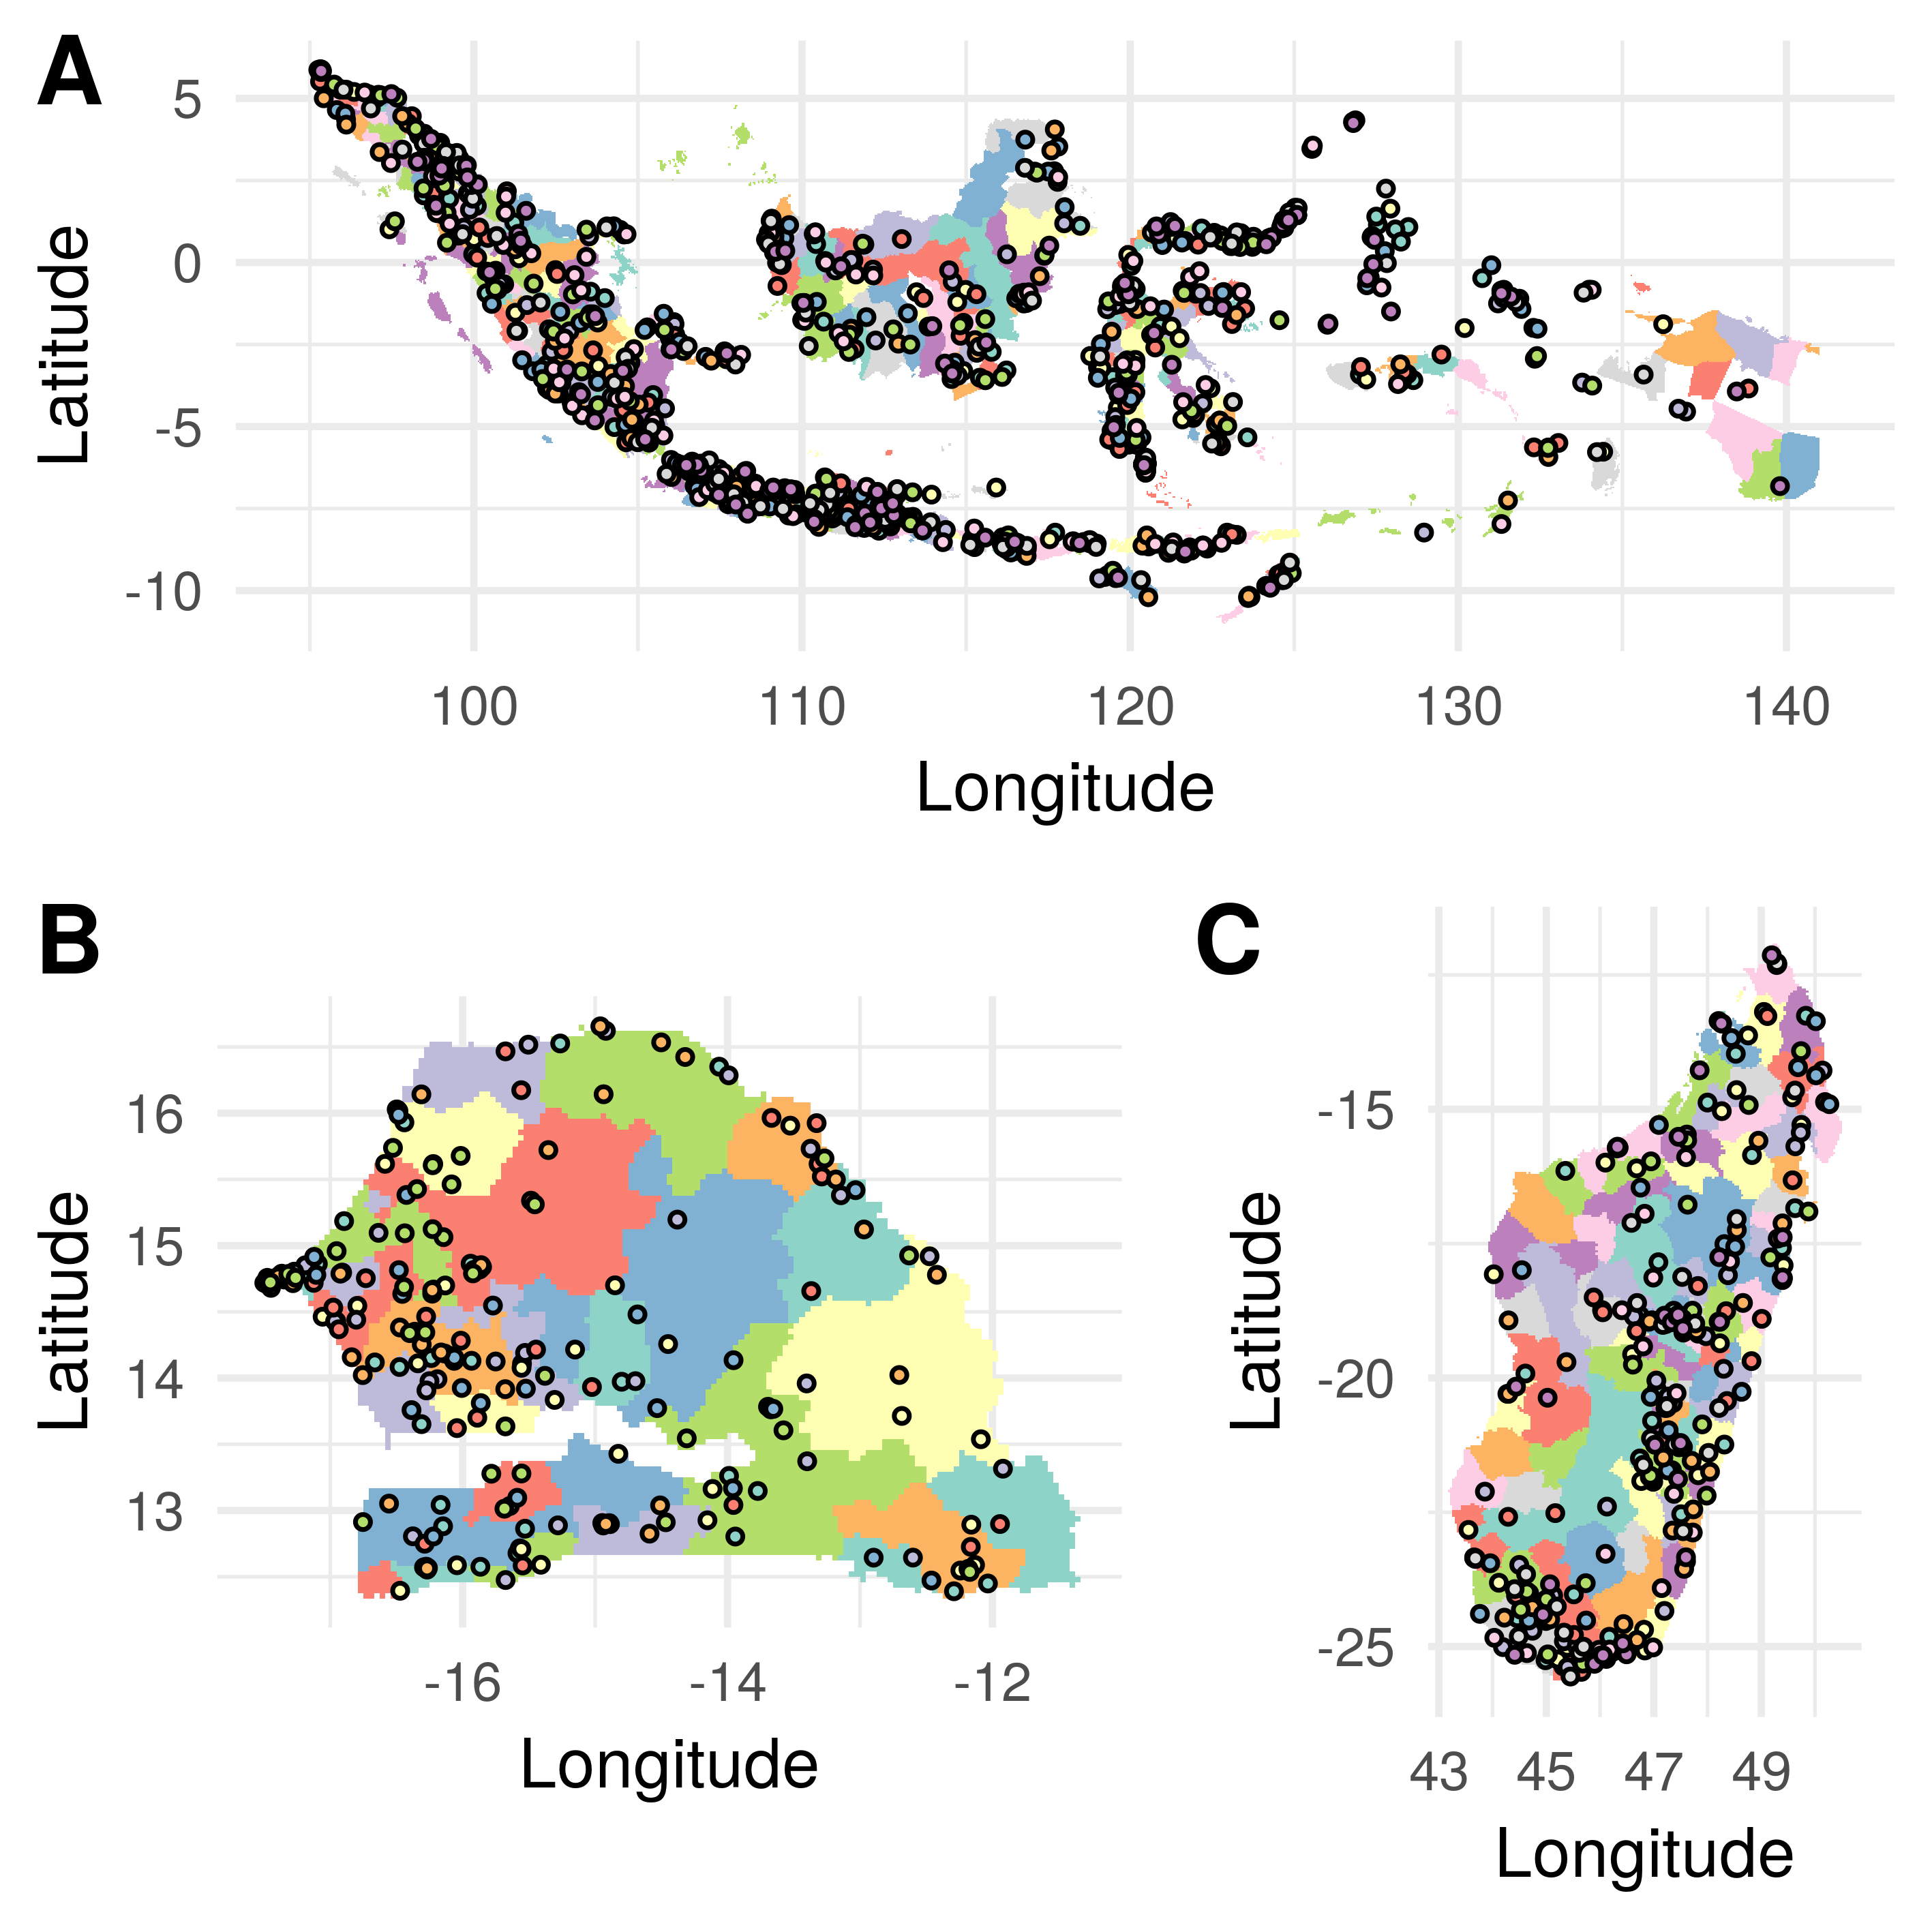
\includegraphics[width = 0.8\textwidth]{figures/random_crossvalidation_full.png} 

\caption{Random cross-validation scheme for Indonesia, Senegal and Madagascar. The fold for both aggregated incidence data and prevalence point data is shown.}
\label{fig:cv_random}
\end{figure}


\begin{figure}[h!]
\centering

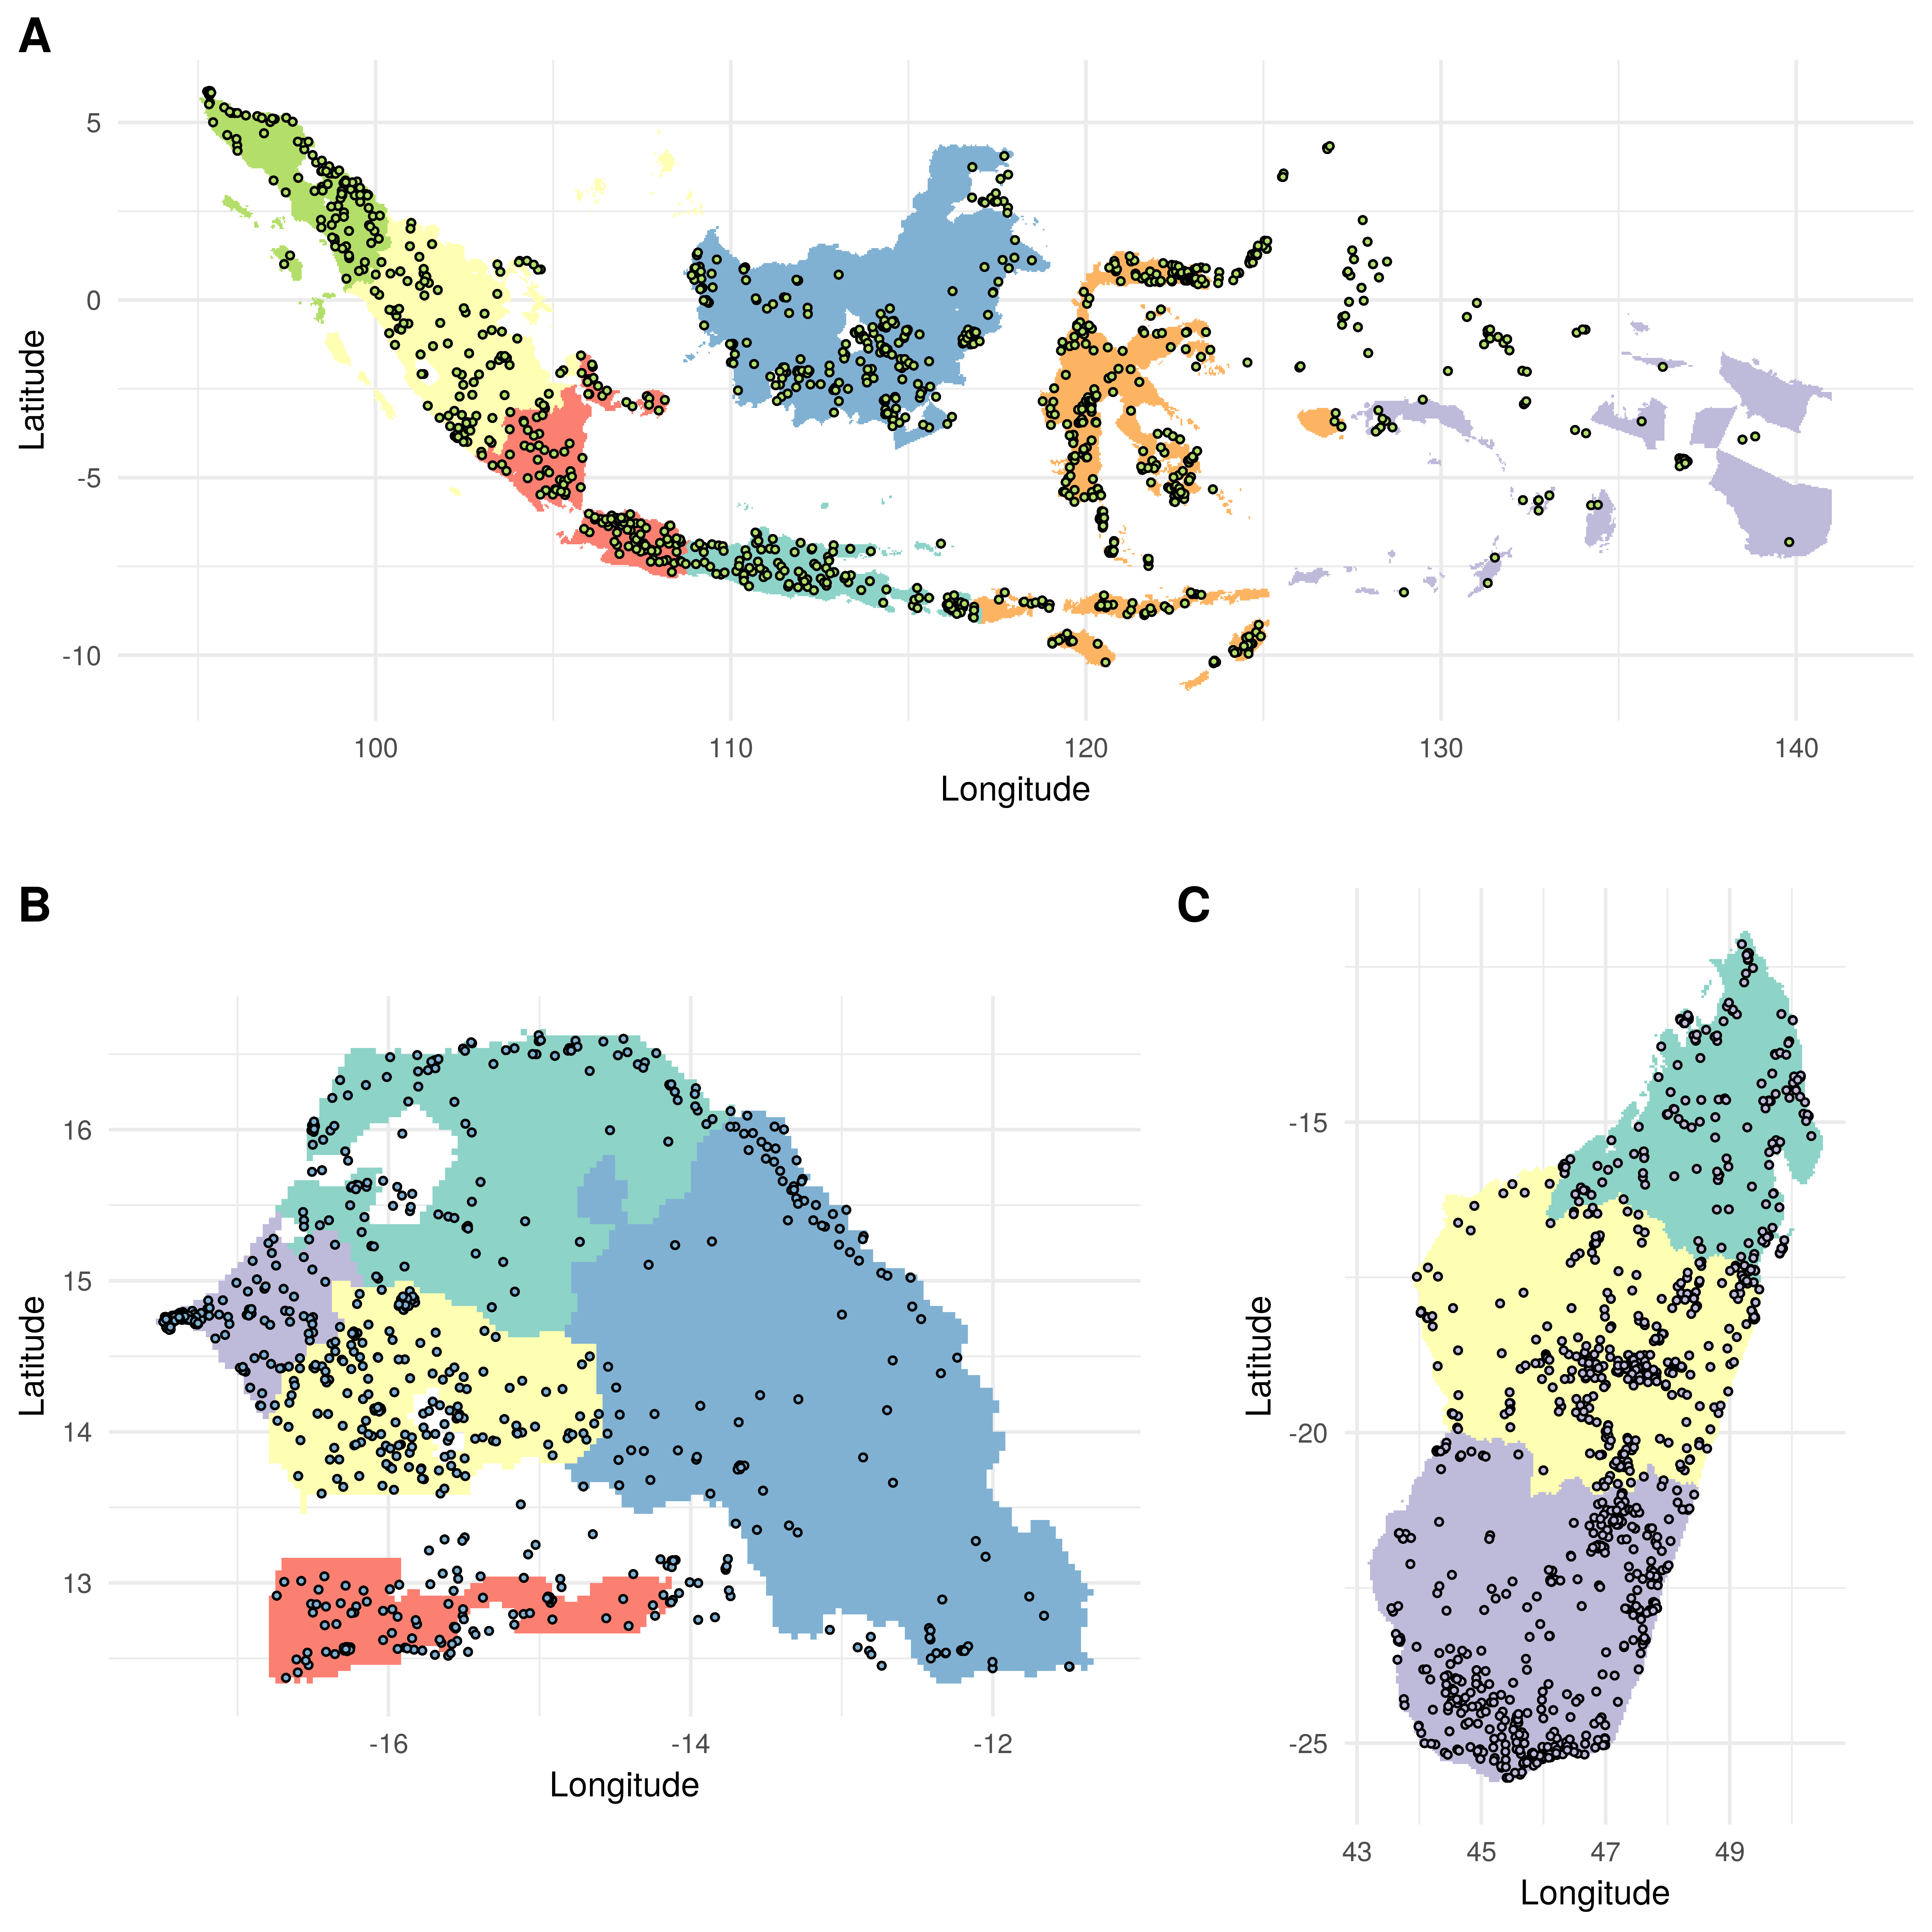
\includegraphics[width = 0.8\textwidth]{figures/spatial_crossvalidation_full.png}

\caption{ Spatial cross-validation scheme for Indonesia, Senegal and Madagascar. The fold for both aggregated incidence data and prevalence point data is shown.}
\label{fig:cv_spatial}
\end{figure}



\clearpage
\section{Estimated parameters}

% latex table generated in R 3.4.4 by xtable 1.8-4 package
% Fri Jul 19 12:48:02 2019
\begin{table}[ht]
\centering
\begin{tabular}{lrrrrrr}
  \hline
Parameters & Baseline & BaselineSD & PrevalenceGP & PrevalenceGPSD & Joint & JointSD \\ 
  \hline
$\beta_0$ & -5.58 & 0.29 & -4.66 & 0.58 & -5.35 & 0.52 \\ 
  $\beta_p$ &  &  &  &  & 1.63 & 0.13 \\ 
  LST day mean & 0.00 & 0.26 & -0.02 & 0.26 & -0.04 & 0.24 \\ 
  EVI & 0.43 & 0.23 & 0.35 & 0.24 & 0.35 & 0.20 \\ 
  TSI & -0.61 & 0.24 & -0.51 & 0.24 & 0.42 & 0.17 \\ 
  accessability & -0.09 & 0.21 & -0.07 & 0.21 & 0.11 & 0.11 \\ 
  elevation & 0.44 & 0.21 & 0.36 & 0.22 & 0.31 & 0.18 \\ 
  LST day SD & 0.23 & 0.20 & 0.07 & 0.21 & 0.24 & 0.20 \\ 
  Night lights & 0.10 & 0.06 & 0.08 & 0.06 & 0.07 & 0.04 \\ 
  TCW & -0.02 & 0.28 & -0.05 & 0.28 & 0.17 & 0.23 \\ 
  Prev GP &  &  & 0.30 & 0.17 &  &  \\ 
  $\omega_v$ & 0.25 & 0.25 & 0.27 & 0.25 & -0.03 & 0.32 \\ 
  $\omega_w$ &  &  &  &  & -1.03 & 0.13 \\ 
  $\log(\sigma_u)$ & -2.48 & 0.61 & -2.53 & 0.63 & -3.35 & 0.52 \\ 
  $\log(\rho)$ & 0.58 & 0.30 & 0.58 & 0.30 & 0.71 & 0.31 \\ 
  $\log(\alpha)$ &  &  &  &  & -0.00 & 0.00 \\ 
   \hline
\end{tabular}
\label{parssen}
\caption[Parameter estimates for Senegal]{Parameter estimates for Senegal. $\omega_v = \log\left(\frac{1}{{\sigma_v}^2}\right)$ and $\omega_w = \log\left(\frac{1}{{\sigma_w}^2}\right)$} 
\end{table}

% latex table generated in R 3.4.4 by xtable 1.8-4 package
% Fri Jul 19 12:48:37 2019
\begin{table}[ht]
\centering
\begin{tabular}{lrrrrrr}
  \hline
Parameters & Baseline & BaselineSD & PrevalenceGP & PrevalenceGPSD & Joint & JointSD \\ 
  \hline
$\beta_0$ & -3.81 & 0.32 & -2.66 & 0.29 & -3.77 & 0.30 \\ 
  $\beta_p$ &  &  &  &  & 0.07 & 0.10 \\ 
  LST day mean & 0.16 & 0.29 & 0.14 & 0.27 & 0.14 & 0.24 \\ 
  EVI & 0.34 & 0.21 & 0.23 & 0.19 & 0.46 & 0.13 \\ 
  TSI & 0.45 & 0.22 & 0.42 & 0.21 & 0.63 & 0.19 \\ 
  accessability & 0.36 & 0.11 & 0.15 & 0.10 & 0.24 & 0.07 \\ 
  elevation & -0.11 & 0.18 & -0.05 & 0.16 & 0.31 & 0.12 \\ 
  LST day SD & -0.22 & 0.21 & -0.15 & 0.17 & -0.20 & 0.15 \\ 
  Night lights & -0.01 & 0.03 & -0.02 & 0.02 & -0.02 & 0.02 \\ 
  TCW & -0.26 & 0.26 & -0.22 & 0.25 & -0.15 & 0.15 \\ 
  Prev GP &  &  & 0.36 & 0.07 &  &  \\ 
  $\omega_v$ & 1.19 & 0.23 & 1.26 & 0.23 & 1.38 & 0.26 \\ 
  $\omega_w$ &  &  &  &  & -0.77 & 0.11 \\ 
  $\log(\sigma_u)$ & -2.57 & 0.60 & -2.83 & 0.63 & -3.21 & 0.49 \\ 
  $\log(\rho)$ & 0.99 & 0.32 & 0.69 & 0.31 & 0.73 & 0.27 \\ 
  $\log(\alpha)$ &  &  &  &  & 0.00 & 0.00 \\ 
   \hline
\end{tabular}
\label{parsmdg}
\caption{Parameter estimates for Madagascar $\omega_v = \log\left(\frac{1}{{\sigma_v}^2}\right)$ and $\omega_w = \log\left(\frac{1}{{\sigma_w}^2}\right)$} 
\end{table}



% latex table generated in R 3.4.4 by xtable 1.8-4 package
% Fri Jul 19 12:48:41 2019
\begin{table}[ht]
\centering
\begin{tabular}{lrrrrrr}
  \hline
Parameters & Baseline & BaselineSD & PrevalenceGP & PrevalenceGPSD & Joint & JointSD \\ 
  \hline
$\beta_0$ & -5.83 & 0.65 & -5.59 & 0.80 & -6.31 & 0.56 \\ 
  $\beta_p$ &  &  &  &  & 0.03 & 0.20 \\ 
  LST day mean & -0.03 & 0.20 & -0.03 & 0.20 & 0.28 & 0.27 \\ 
  EVI & 0.11 & 0.08 & 0.11 & 0.08 & 0.55 & 0.18 \\ 
  TSI & 0.24 & 0.19 & 0.24 & 0.19 & -0.02 & 0.24 \\ 
  accessability & 0.73 & 0.24 & 0.73 & 0.24 & 0.36 & 0.19 \\ 
  elevation & -0.12 & 0.12 & -0.12 & 0.12 & -0.23 & 0.22 \\ 
  LST day SD & 0.04 & 0.11 & 0.04 & 0.11 & -0.04 & 0.18 \\ 
  Night lights & -0.34 & 0.12 & -0.34 & 0.12 & 0.01 & 0.10 \\ 
  TCW & 0.05 & 0.10 & 0.05 & 0.10 & 0.06 & 0.19 \\ 
  Prev GP &  &  & 0.06 & 0.12 &  &  \\ 
  $\omega_v$ & -1.54 & 0.11 & -1.54 & 0.11 & -1.33 & 0.11 \\ 
  $\omega_w$ &  &  &  &  & -2.65 & 0.09 \\ 
  $\log(\sigma_u)$ & -2.23 & 0.43 & -2.25 & 0.43 & -2.79 & 0.48 \\ 
  $\log(\rho)$ & 1.63 & 0.23 & 1.62 & 0.23 & 1.38 & 0.24 \\ 
  $\log(\alpha)$ &  &  &  &  & -0.00 & 0.00 \\ 
   \hline
\end{tabular}
\label{parsidn}
\caption{Parameter estimates for Indonesia $\omega_v = \log\left(\frac{1}{{\sigma_v}^2}\right)$ and $\omega_w = \log\left(\frac{1}{{\sigma_w}^2}\right)$} 
\end{table}






\begin{figure}
% to be removed before submission
\makebox{\includegraphics[width = 1.05\textwidth]{figures/random_cv_poly_facet.pdf}  }
\caption{\label{randompredobspolyfacet} 
Observed-predicted plots (square root scale) of modelled annual malaria incidence (cases per 1000) by country from the random cross-validation experiments for Indonesia (Panel A), Senegal (Panel B) and Madagascar (Panel C). 
Results from the baseline disaggregation model are shown in red, the prevalence GP model is shown in green while the joint model is shown in blue.
The one-one line is shown with a black line and a simple linear regression through the points is shown by a coloured line.
}

\end{figure}




\clearpage
\section{Cross-validation predictions}


\begin{figure}[h!]
% to be removed before submission
\makebox{\includegraphics[width = 0.7\textwidth]{figures/idn_both_cv12_random_preds.png}}
\caption{\label{predobsmapsen1}
Incidence data and predicted incidence maps.
The incidence (log10) data (top), predicted log10 incidence from the prevalence GP model for random cross-validated out-of-sample polygons (middle) and predicted log10 incidence from the joint model for spatially cross-validated out-of-sample polygons (bottom) for Senegal.
}
\end{figure}



\begin{figure}[h!]
% to be removed before submission
\makebox{\includegraphics[width = 0.9\textwidth]{figures/mdg_both_cv12_random_preds.png}}
\caption{\label{predobsmapsen2}
Incidence data and predicted incidence maps.
The incidence (log10) data (top), predicted log10 incidence from the prevalence GP model for random cross-validated out-of-sample polygons (middle) and predicted log10 incidence from the joint model for spatially cross-validated out-of-sample polygons (bottom) for Senegal.
}
\end{figure}



\begin{figure}[h!]
% to be removed before submission
\makebox{\includegraphics[width = 1\textwidth]{figures/sen_both_cv12_random_preds.png}}
\caption{\label{predobsmapsen3}
Incidence data and predicted incidence maps.
The incidence (log10) data (top), predicted log10 incidence from the prevalence GP model for random cross-validated out-of-sample polygons (middle) and predicted log10 incidence from the joint model for spatially cross-validated out-of-sample polygons (bottom) for Senegal.
}
\end{figure}



\clearpage
\subsection{Full model predictions}
\subsubsection{Madagascar}

\begin{figure}[h!]
\centering

\includegraphics[width = 0.3\textheight]{figures/mdg_baseline_api.png}

\caption{Predictions from the baseline model fitted to all data in Madagascar.}
\label{baselinemdg}
\end{figure}
\begin{figure}[h!]
\centering

\includegraphics[width = 0.3\textheight]{figures/mdg_prgp_api.png}

\caption{Predictions from the prevalence GP model fitted to all data in Madagascar.}
\label{gpmdg}
\end{figure}

\begin{figure}[h!]
\centering

\includegraphics[width = 0.3\textheight]{figures/mdg_joint_api.png}

\caption{Predictions from the joint model fitted to all data in Madagascar.}
\label{jointmdg}
\end{figure}




\subsubsection{Senegal}


\begin{figure}[h!]
\centering

\includegraphics[width = 0.3\textheight]{figures/sen_baseline_api.png}

\caption{Predictions from the baseline model fitted to all data in Senegal.}
\label{baselinesen}
\end{figure}
\begin{figure}[h!]
\centering

\includegraphics[width = 0.3\textheight]{figures/sen_prgp_api.png}

\caption{Predictions from the prevalence GP model fitted to all data in Senegal.}
\label{gpsen}
\end{figure}

\begin{figure}[h!]
\centering

\includegraphics[width = 0.3\textheight]{figures/sen_joint_api.png}

\caption{Predictions from the joint model fitted to all data in Senegal.}
\label{jointsen}
\end{figure}



\subsubsection{Indonesia}


\begin{figure}[h!]
\centering

\includegraphics[width = 0.5\textheight]{figures/idn_baseline_api.png}

\caption{Predictions from the baseline model fitted to all data in Indonesia.}
\label{baselineidn}
\end{figure}
\begin{figure}[h!]
\centering

\includegraphics[width = 0.5\textheight]{figures/idn_prgp_api.png}

\caption{Predictions from the prevalence GP model fitted to all data in Indonesia.}
\label{gpidn}
\end{figure}

\begin{figure}[h!]
\centering

\includegraphics[width = 0.5\textheight]{figures/idn_joint_api.png}

\caption{Predictions from the joint model fitted to all data in Indonesia.}
\label{jointidn}
\end{figure}







\clearpage

\subsection{Full model fields}


\subsubsection{Senegal}




\begin{figure}[h!]
\centering

\includegraphics[width =  0.3\textheight]{figures/sen_baseline_field.png}

\caption{The random field as fitted to all the data in the baseline model.}
\label{baselinefieldsen}
\end{figure}


\begin{figure}[h!]
     \centering
     \subfloat[][The prevalence GP model that is used as a covariate.]{\includegraphics[width = 0.3\textheight]{figures/sen_prevgp.png}}
     \subfloat[][The random field as fitted to all the data in the prevalence GP model.]{\includegraphics[width = 0.3\textheight]{figures/sen_prgp_field.png}}
     \label{gpsencov}
\end{figure}
%remaining part


\begin{figure}[h!]
\centering

\includegraphics[width =  0.3\textheight]{figures/sen_joint_field.png}

\caption{The random field as fitted to all the data in the joint model.}
\label{jointfieldsen}
\end{figure}




\clearpage
\subsubsection{Indonesia}




\begin{figure}[h!]
\centering

\includegraphics[width =  0.6\textheight]{figures/idn_baseline_field.png}

\caption{The random field as fitted to all the data in the baseline model.}
\label{baselinefieldidn}
\end{figure}



\begin{figure}[h!]
     \centering
     \subfloat[][The prevalence GP model that is used as a covariate.]{\includegraphics[width =0.5\textwidth ]{figures/idn_prevgp.png}}
     \subfloat[][The random field as fitted to all the data in the prevalence GP model.]{\includegraphics[width = 0.5\textwidth]{figures/idn_prgp_field.png}}
     \label{gpsencov}
\end{figure}
%remaining part

\begin{figure}[h!]
\centering

\includegraphics[width =  0.6\textheight]{figures/idn_joint_field.png}

\caption{The random field as fitted to all the data in the joint model.}
\label{jointfieldidn}
\end{figure}



\clearpage
\subsubsection{Madagascar}





\begin{figure}[h!]
\centering

\includegraphics[width =  0.3\textheight]{figures/mdg_baseline_field.png}

\caption{The random field as fitted to all the data in the baseline model.}
\label{baselinefieldmdg}
\end{figure}




\begin{figure}[h!]
     \centering
     \subfloat[][The prevalence GP model that is used as a covariate.]{\includegraphics[width =0.5\textwidth ]{figures/mdg_prevgp.png}}
     \subfloat[][The random field as fitted to all the data in the prevalence GP model.]{\includegraphics[width = 0.5\textwidth]{figures/mdg_prgp_field.png}}
     \label{gpsencov}
\end{figure}
%remaining part




\begin{figure}[h!]
\centering

\includegraphics[width =  0.3\textheight]{figures/mdg_joint_field.png}

\caption{The random field as fitted to all the data in the joint model.}
\label{jointfieldidn}
\end{figure}


\end{document}
